\newpage
\section{Билет 10. Понятие температуры. Теплопроводность. Цикл Карно. Абсолютная температура. КПД цикла Карно. Второе начало термодинамики. Энтропия.}



\begin{center}
	\textit{\underline{Понятие температуры}}
\end{center}

Мы говорим, что тело А имеет большую, чем тело В, температуру ($T_A > T_B$), если при контакте тела А с телом В возникает переход тепловой энергии от тела А к телу В. Понятие температуры не имеет смысла в аналитической механике для систем с небольшим числом степеней свободы. На практике температуру можно приписывать телам, состоящим из большого числа частиц. 

Из молекулярно-кинетической теории известно, что температуру можно рассматривать как величину, пропорциональную средней энергии хаотического теплового движения молекул, приходящуюся на одну степень свободы молекулы.  Температура не иммет смысла для неравновесных систем, в которых не успевает происходить выравнивание (планета).  Обычно рассматривают температуру достаточно малых частей тела и изучают тепловые потоки в теле. Опыт показывает, что во многих практических вопросах часто можно предполагать, что термодинамическое равновесие в малых объемах системы имеет место.  


\begin{center}
	\textit{\underline{Теплопроводность}}
\end{center}

Теплопроводность - способность материальных тел проводить тепловую энергию от более нагретых частей тела к менее нагретым частям тела. Опыт показывает, что для многих сред для вектора потока тепла $\vec{q}$ выполняется закон теплопроводности Фурье. Для изотропной среды этот закон утверждает, что вектор потока тепла $\vec{q}$ пропорционален градиенту температуры T: $$\vec{q} = -\kappa grad T, \, aka \, q_i = -\kappa \frac{\partial T}{\partial x^i},$$ где $\kappa$ - коэффициент теплопроводности. Для анизотропной среды: $$q_i = -\kappa^{ij} \frac{\partial T}{\partial x^i},$$ $\kappa^{ij}$ - компоненты тензора коэффициентов теплопроводности.
Двухпараметрической средой называется среда, все термодинамические функции которой зависят только от двух термодинамических параметров состояния. Если эти два параметра - давление р и плотность $\rho$, то удельная внутренняя энергия такой среды должна выражаться через них: $U = U (p, \rho)$.

Если среда представляет собой идеальную сжимаемую жидкость (гаа), то работа внутренних поверхностных сил, отнесенная к единице массы, имеет вид
$$ \frac{1}{dm}dA_{face}^{(i)} = p\ d\frac{1}{\rho} $$
и уравнение притока тепла в предположении, что $q^{**} = 0$ записывается следующим образом:
$$ dU + p\ d\frac{1}{\rho} = dq^{(e)} $$

В совершенном газе давление, плотность и темцература связаны уравнением Клапейрона:
$$ p = \rho R T $$

R - некоторое постоянное число, называемое газовойпостоянной, различное для разных газов. Уравнение этого типа, связывающее давление, температуру, плотность и, возможно, другие физические характеристики среды, называется уравнением состояния.

Можно ввести ушиверсальную (постоянную для всех газов) газовую постоянную R. и постоянную Больцмана к согласно равенствам
$$ R = \frac{R_0}{M} = \frac{k}{m} $$

Здесь М- - средняя масса одной грамм-молекулы газа, определяемая по формуле
$$ \frac{n}{M} = \frac{n_1}{M_1} + ... + \frac{n_k}{M_k} $$

где k - полное число молекул в данном обьеме смеси,  $n_i$ число молекул, а $M_i$ - соответствующие массы грамм-молекул отдельных сортов газов; m - средняя масса молекулы в граммах.

Совершенный газ можно определить как газ, в котором молекулы взаимодействуют только при столкновениях. Поэтому можно считать, что внутренняя энергия одноатомного соверщенного газа представляет собой суммарную кинетическую ёнергию хаотического движения атомов. 

Для внутренней энергии U единицы массы можно написать
$$ U = \frac{1}{M}\sum\limits_{i=1}^{N}\frac{m_iv_i^2}{2} + const $$

Если считать, что все атомы газа одинаковые, то $M = Nm$ и 
$$ U = \frac{v_{average}^2}{2} + const $$

Для совершенного газа, согласно определению температуры как характеристики средней энергии, приходящейся на одну степень свободы в хаотическом тепловом движении атомов, удельную внутреннюю энергию U можно представить в виде
$$ U = c_VT + const \ \ \ \ (*)$$

Здесь через $c_V$ обозначен размерный коэффициент пропорциональности между $\frac{1}{2}v_{average}^2$ и T

Задание внутренней энергии U в виде $(*)$ вместе с уравнением Клапейрона фиксирует определенную модель сплошной среды, называемую совершенным газом. Сравнения с экспериментальными данными показывают, что движения реальных газов при обычных условиях достаточно хорошо описываются такой моделью.

На основании уравнения притока тепла для совершенного идеального газа в случае процесса, протекающего при постоянном удельном объеме $\left(\displaystyle d\frac{1}{\rho}=0\right)$ можно легко получить, что
$$ (dq^{(e)})_{V = const} = dU = c_VdT $$
или
$$ \left( \frac{dq^{(e)}}{dT} \right)_{V=const} = c_V $$

Следовательно,  $c_V$ представляет собой количество тепла,которое необходимо подвести к единице массы среды для того, чтобы при постоянном объеме поднять ее температуру на $1^oC$;  поэтому $c_V$ называется теплоемкостью при постоянном объеме.

В случае процесса при постоянном давлении из уравнения притока тепла для идеального совершенного газа получим
$$ \left(d q^{(e)}\right)_{p=\text { const }}=d U+p d \frac{1}{\rho}=c_V d T+d \frac{p}{\rho}=\left(c_V+R\right) d T $$

Количество тепла, которое необходимо подвести к единице мас- сы среды, чтобы при постоянном давлении поднять температу- ру на $1^oC$, называется теплоемкостью при постоянном давлении и обозначается через $C_p$:
$$ c_p = \left( \frac{dq^{(e)}}{dT} \right)_{p=const} $$

Следовательно, $$ c_p - c_V = R $$


\begin{center}
	\textit{\underline{Цикл Карно}}
\end{center}

Процесс \textbf{адиабатический}, если в нем отсутствует приток внешнего тепла и теплообмен между соседними частицами. Т.е. $\displaystyle dQ^{(e)} = 0$
Процесс \textbf{изотермический}, если теплообмен, обусловленный теплопроводностью или излучением, пред- ставляет собой настолько интенсивный продесс, а изменение состояний протекает настолько медленно, что температуру всех частей системы можно считать постоянной. Т.е. $\displaystyle \frac{dT}{dt} = 0$

Рассмотрим следующий важный равновесный обратимый замкнутый процесс, который носит название обратимого цикла Карно. Рабочим телом, т. е. средой, которая совершает этот цикл, пусть будет совершенный газ или любая другая двухпараметрическая среда - определяемая параметрами р и $\frac{1}{\rho}$. 

Из произвольной точки $M (p_0, \frac{1}{\rho_0})$ пространства состояний газ по изотерме $\theta_1 = const$ бесконечно медленно расширяется до состояния $N$, затем газ расширяется адиабатически до состояния $K$ с  температурой $\theta_2 < \theta_1$ и от $K$ сжимается изотермически до состояния $P$, из которого можно вновь вернуться по адиабате в первоначальное состояние $M$.

\begin{figure}[H]
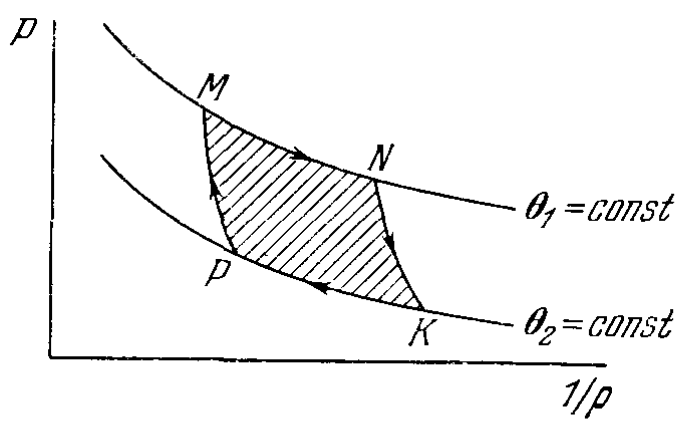
\includegraphics[width=0.7\textwidth]{10/carno.png}
\end{figure}


\begin{center}
	\textit{\underline{Второй закон термодинамики}}
\end{center}

\textbf{Формулировка 1:} Невозможно устройство, которое переводило бы тепло от тела с меньшей температурой к телу с большей температурой без каких-либо изменений в других телах.

\textbf{Формулировка 2:} нельзя построить так называемый вечный двигатель второго рода, т.е. машину,  которая,  работая в согласии с первым законом термодинамики по некоторому циклу,  периодически совершала бы работу только за счет охлаждения некоторого одного и того же источника тепла с фиксированной температурой (отбор тепла из резервуара с постоянной температурой).

$$ A = Q_1 - Q_2 $$

Введем понятие коэффициента полезного действия (к.п.д.) $\eta$ тепловой машины, работающей по циклу Карно. По определению к.п.д.  цикла Карно называется отношение полученной в результате реализации цикла механической работы $А > 0$ к подведенному к системе за время цикла теплу $Q_1 > 0$.  Для к. п. д. цикла Карно верна формула
$$ \eta = \frac{A}{Q_1} = 1 - \frac{Q_2}{Q_1} < 1 $$

Полученной свойство $\eta < 1$ есть следствие первого закона термодинамики. 

\begin{state}
	Для всякого обратимого цикла Карно величина $\eta$ зависит только от температур $\theta_1$ и $\theta_2$,  заданных на изотермах $MN$ и $KP$ и не зависит ни от свойств рабочего тела, участвующего в цикле Карно ни от способа организации цикла, определяемого, например, размерами рабочего тела и степенью расширения вдоль изотерм.
\end{state}

Докажем, что $\eta$ зависит только от $\theta_1$ и $\theta_2$ и является абсолютной характеристикой обратимого цикла Карно, т. е. универсальной функцией $\eta(\theta_1, \theta_2)$. Одновременнос этим покажем,  что еслит емпературы $\theta_1$ и $\theta_2$ фиксированы,то к. п. д. $\eta'$ машины,  работающей по необратимому циклу Карно не может быть больше к. п. д.  $\eta$ машины, работающей по соответствующему обратимому циклу Карно, т. е.
$$ \eta' \leq \eta $$
\begin{proof}
(От противного, противоречие со вторым законом термодинамики):

Пусть есть 2 цикла - обратимый ($\eta$) и необратимый ($\eta'$) c одинаковыми температурами $\theta_1 > \theta_2$. Пусть $\eta' > \eta$. Пусть машина с к.п.д. $\eta'$ работает в прямом направлении и проивзодит работу $A'$. Заставим обратимую машину работать в противоположном направлении (холодильная машина).  Тогда для машины с к.п.д. $\eta'$ имеем $Q'_1 > 0$, $Q'_2 > 0$ и $A' = Q'_1 - Q'_2 > 0$.  А для машины с к.п.д. $\eta$ имеем $Q_1 > 0$, $Q_2 > 0$ и $A = Q_2 - Q_1 < 0$. Выберем обратимый цикл Карно так, чтобы имело место равенство $-A = A'$, т.е. $Q_1' - Q_2' = Q_1 - Q_2$ и соединим эти машины вместе. Получим машину, для которой $$ A_0 = A' + A = Q_1 + Q_2 - Q_1' - Q_2' $$

Единственный эффект, производимый этой составной машиной, будет заключаться в перераспределении теплоты между телами,  которые служат нагревателем и холодильником.

По построению (по выбору машин): $|A| = A' \ \ \Rightarrow \eta Q_1 = \eta'Q_1' $. Значит из предположения $\eta' > \eta$ следует $$ Q_1' < Q_1 $$
или $$ Q_1 - Q_1' = Q_2 - Q_2' > 0 $$
Здесь слева количество тепла,  передаваемое в резервуар с более высокой температурой, а справа - равна общему количеству тепла, забираемому из резервуара с температурой $\theta_2$

Таким образом, составная машина без затраты внешней энергии будет переводить тепло от холодного резервуара к горячему, что невозможно согласно второму закону термодинамики.

\end{proof} 

При доказательстве мы не пользовались ни свойствами рабочего тела ни частными свойствами цикла, следовательно, к.п.д.  обратимого цикла Карно не зависит от свойств рабочего вещества и от степени расширения,  а зависит только от $\theta_1$ и $\theta_2$ и является универсальной функцией $\eta = \eta(\theta_1, \theta_2)$

Найдем эту универсальную функцию.  По определению к.п.д. цикла Карно имеем
$$ \eta(\theta_1, \theta_2) = \frac{A}{Q_1} = 1 - \frac{Q_2}{Q_1} $$
Введем функцию $f(\theta_1, \theta_2) = 1 - \eta(\theta_1, \theta_2) = \frac{Q_2}{Q_1}$

Рассмотрим три тела большой теплоемкости с температурами $\theta_1, \theta_2, \theta_3$ и три обратимых цикла Карно, в которых эти тела служат нагревателями или холодильниками.
$$ f(\theta_1, \theta_2) = \frac{Q_2}{Q_1} = \frac{Q_2}{Q_3}\frac{Q_3}{Q_1} = f(\theta_3, \theta_2)f(\theta_1, \theta_3) $$

В случае $\theta_1 = \theta_2$:
$$ 1 = f(\theta_3, \theta_1)f(\theta_1, \theta_3) $$
То есть при перестановке аргументов функция обращается. Следваотельно, 
$$ \frac{Q_2}{Q_1} = f(\theta_1, \theta_2) = \frac{f(\theta_3, \theta_2)}{f(\theta_3, \theta_1)} \ \ \ \ (**)$$
Отсюда следует, что $\frac{Q_2}{Q_1}$ не зависит от $\theta_3$.  Решение функционального уравнения $(**)$ имеет вид
$$ f(\theta_1, \theta_2) = \frac{\omega(\theta_2)}{\omega(\theta_1)} $$
Следовательно $$ \frac{Q_2}{Q_1} = \frac{\omega(\theta_2)}{\omega(\theta_1)} $$

\begin{defn}
	Абсолютная температура $T$ - значение функции $\omega(\theta)$
\end{defn}

Тогда $$ \frac{Q_2}{Q_1} = \frac{T_2}{T_1} $$

\textbf{Формулировка 3 (количественная для обратимого цикла Карно):} 
$$ \frac{Q_1^{(e)}}{T_1} + \frac{Q_2^{(e)}}{T_2} = 0 $$


\begin{center}
	\textit{\underline{Энтропия}}
\end{center}

Фиксируя точку начального состояния системы А для любого состояния В двупараметрической среды, в которое можно перейти из состояния А обратимыми путями, можно ввести функцию параметров состояния - координат точки В:
$$ S(B) = S\left(p, \frac{1}{\rho}\right) = \int\limits_{A}^{B}\frac{dQ^{(e)}}{T} + S(A) $$

\begin{defn}
	 Энтропия - это функция $S(B)$
\end{defn}

Из определения следует, что $$ dS = \frac{dQ^{(e)}}{T} $$
Из уравнения притока тепла:
$$ dS = \frac{dU_m + dA^{(i)}}{T} $$
Или в рассчете на единицу массы:
$$ ds = \frac{dq^{(e)}}{T} = \frac{dU + pd\frac{1}{\rho}}{T} $$

\textbf{Случай совершенного газа:}

для совершенного газа с постоянными теплоемкостями ($p = \rho R T, \ \ U = c_V T$) будем иметь
$$ ds = \frac{c_VdT}{T} + \frac{Rd\frac{1}{\rho}}{\frac{1}{\rho}} = dln\left[T^{c_V}\left( \frac{1}{\rho} \right)^{R}\right] $$


